\documentclass[tikz,border=2pt]{standalone}
\usepackage{amsmath,amssymb}
\usepackage{pgfplots}
\pgfplotsset{compat=1.18}

\begin{document}
% The N(mu, sigma^2) bell curve: symmetric about mu, inflection points at mu +- sigma, and
% about 68% of the mass within one standard deviation of the mean.
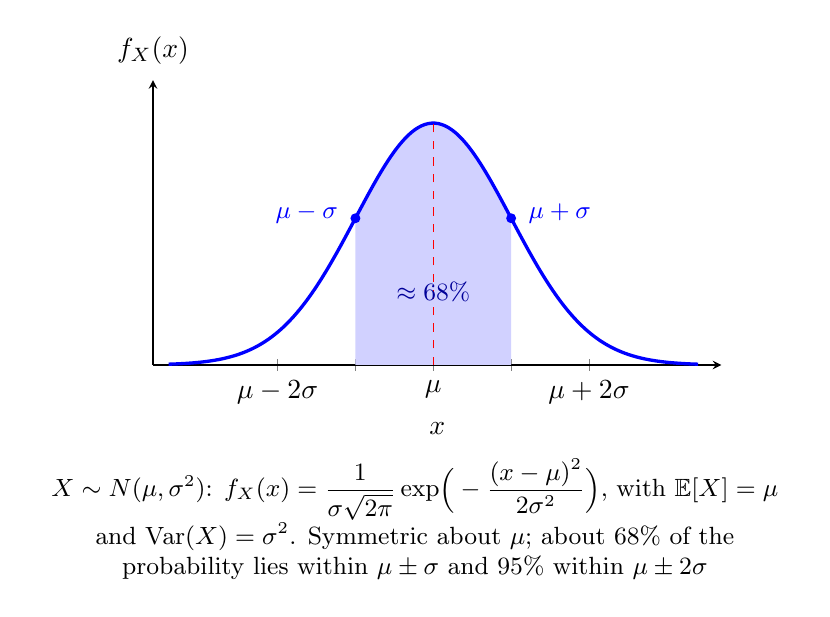
\begin{tikzpicture}
	\begin{axis}[
		axis lines=left, xmin=-1.6, xmax=5.7, ymin=0, ymax=0.47,
		xtick={0,1,2,3,4}, xticklabels={$\mu-2\sigma$,,$\mu$,,$\mu+2\sigma$}, ytick=\empty,
		xlabel={$x$}, ylabel={$f_X(x)$}, ylabel style={rotate=-90, anchor=south, at={(axis description cs:0,1.02)}},
		samples=160, smooth, width=8.8cm, height=5.2cm, clip=false
		]
		\addplot[fill=blue!18, draw=none, domain=1:3] {exp(-(x-2)^2/2)/sqrt(2*pi)} \closedcycle;
		\addplot[blue, very thick, domain=-1.4:5.4] {exp(-(x-2)^2/2)/sqrt(2*pi)};
		\draw[red, dashed] (axis cs:2,0) -- (axis cs:2,0.399);
		\fill[blue] (axis cs:1,0.242) circle (1.8pt);
		\fill[blue] (axis cs:3,0.242) circle (1.8pt);
		\node[blue, font=\small, anchor=east] at (axis cs:0.9,0.25) {$\mu-\sigma$};
		\node[blue, font=\small, anchor=west] at (axis cs:3.1,0.25) {$\mu+\sigma$};
		\node[blue!60!black, font=\small] at (axis cs:2,0.12) {$\approx68\%$};
	\end{axis}
	\node[anchor=north, font=\small, align=flush center, text width=9.6cm] at ([yshift=-2pt]current axis.outer south) {$X\sim N(\mu,\sigma^2)$: $f_X(x)=\dfrac1{\sigma\sqrt{2\pi}}\exp\!\Big(-\dfrac{(x-\mu)^2}{2\sigma^2}\Big)$, with $\mathbb{E}[X]=\mu$ and $\operatorname{Var}(X)=\sigma^2$. Symmetric about $\mu$; about $68\%$ of the probability lies within $\mu\pm\sigma$ and $95\%$ within $\mu\pm2\sigma$};
\end{tikzpicture}
\end{document}
